\documentclass[11pt]{article}

% --- Geometry ---
\usepackage[margin=1in]{geometry}

% --- Encoding & fonts ---
\usepackage[utf8]{inputenc}
\usepackage[T1]{fontenc}
\usepackage{lmodern}

% --- Math ---
\usepackage{amsmath,amssymb}

% --- Tables ---
\usepackage{booktabs}
\usepackage{multirow}
\usepackage{array}

% --- Figures ---
\usepackage{graphicx}
\usepackage{subcaption}
\usepackage[dvipsnames]{xcolor}

% --- Hyperlinks ---
\usepackage[breaklinks=true,colorlinks=true,linkcolor=blue,citecolor=blue,urlcolor=blue]{hyperref}

% --- Bibliography ---
\usepackage{natbib}
\bibliographystyle{plainnat}

% --- Misc ---
\usepackage{enumitem}
\usepackage{microtype}

% --- Title ---
\title{TaskBench: Measuring Cost-Quality Tradeoffs\\Across 46 LLMs and 21 Production Tasks}
\author{S\'{e}bastien Conejo}
\date{}

\begin{document}
\maketitle

% ============================================================
% ABSTRACT
% ============================================================
\begin{abstract}
We benchmark 46 large language models from 12 API providers across 21
production tasks spanning sentiment classification, intent detection,
code generation, mathematical reasoning, and 17 others.  We measure both
per-query cost and quality on 50 cases per task (51,580 scored cases
total).  Economy-tier models (\$0.05--\$0.49/M input tokens) show no
statistically significant quality gap versus Premium models (\$5+/M) on
19 of 21 tasks (Mann-Whitney $p > 0.05$; $n_{\text{Premium}} = 2$).  Within providers, paying 750$\times$ more
buys at most $+0.13$ quality points on a 1--5 scale.  Per-task routing
to the cheapest adequate model reduces cost by 99.7\% versus the best
single model with negligible quality loss.  Quality scores are produced by an LLM judge
validated against ground truth on three task types
($r = 0.89$--$0.91$).  We release the full dataset, raw model responses,
and evaluation prompts.\footnote{Data and code:
\url{https://github.com/SebConejo/benchmark-reverse-engineering}}
\end{abstract}

% ============================================================
% 1. INTRODUCTION
% ============================================================
\section{Introduction}

\subsection{The Problem}

Practitioners choose large language models by reputation or leaderboard
rank.  Existing benchmarks measure capability along a single axis: MMLU
\citep{hendrycks2021mmlu} tests academic knowledge, Chatbot Arena
\citep{chiang2024chatbot} aggregates human preference into a single Elo
score, and HELM \citep{liang2023helm} evaluates multiple metrics but not
cost.  A model ranked first on Arena may cost 100$\times$ more than the
fifth-ranked model for identical quality on sentiment classification.  No
public dataset lets a practitioner answer a concrete question: for this
specific task, which model gives adequate quality at the lowest cost?

\subsection{Contributions}

We make three contributions.

\begin{enumerate}[leftmargin=*,itemsep=2pt]
\item \textbf{TaskBench}, a public benchmark measuring per-task
  cost-quality Pareto frontiers across 46 models, 21 production tasks,
  12 providers, and 4 price tiers (51,580 scored cases).
\item \textbf{Empirical findings.}  Economy-tier models show no
  significant quality gap versus Premium on 19 of 21 tasks.  Per-task routing
  saves 99.7\% versus the best single model.  Within-provider price
  gradients are nearly flat.
\item \textbf{Judge validation.}  We show that standard LLM-as-judge
  evaluation with generic rubrics has format bias ($r = 0.39$ versus
  ground truth), fix it with correctness-focused rubrics ($r = 0.91$),
  and release both score versions for reproducibility.
\end{enumerate}

We release all raw responses, scores, and evaluation code.

\subsection{Key Findings Preview}

Four headline results:

\begin{itemize}[leftmargin=*,itemsep=2pt]
\item \textit{No Economy--Premium gap detected.}  Mann-Whitney $p > 0.05$
  on 19 of 21 tasks (the two significant results favor opposite tiers).
  Premium averages 4.791 versus Economy 4.741, a gap of 0.050 on the
  1--5 scale.
\item \textit{Flat provider gradients.}  Anthropic Haiku (\$0.80/M)
  scores 4.775 while Opus (\$15/M) scores 4.753.  Google Flash
  (\$0.15/M) matches Pro (\$1.25/M).  OpenAI's 750$\times$ price range
  yields $+0.13$ quality.
\item \textit{Per-task routing saves 99.7\%.}  The cheapest adequate
  model per task averages \$0.000009/query versus \$0.003332 for o3
  alone, with at most 0.2 points quality difference on any task.
\item \textit{Five Economy models cover all tasks.}  At the 4.5/5
  quality threshold, five models cover all 21 tasks.  The cheapest is
  Grok~4~Fast at \$0.000435/query average.
\end{itemize}


% ============================================================
% 2. RELATED WORK
% ============================================================
\section{Related Work}

\subsection{General LLM Benchmarks}

HELM \citep{liang2023helm} evaluates 30 models across 42 scenarios on
7 metric families, but cost is not among them.  Chatbot Arena
\citep{chiang2024chatbot} collects over 1.5 million human preference
votes, yet produces a single aggregate ranking without per-task
granularity.  MMLU \citep{hendrycks2021mmlu} and its successor MMLU-Pro
test academic knowledge rather than production tasks.  The Berkeley function calling benchmark covers a single task type.  TaskBench adds
cost as a first-class evaluation axis and provides per-task granularity
across 21 diverse production tasks.

\subsection{Cost-Aware LLM Evaluation and Routing}

FrugalGPT \citep{chen2023frugalgpt} introduced LLM cascading for cost
reduction but evaluated on one task with three models.  RouterBench and
RouteLLM benchmark router systems, not the underlying models.
RouterArena \citep{lu2025routerarena} evaluates 14 routers on 8{,}400
queries but does not provide per-task cost-quality data for the models
themselves.  Artificial Analysis tracks speed and aggregate pricing but
not per-task quality.  We produce the underlying per-task cost-quality
data that any routing system can consume.

\subsection{LLM-as-Judge}

MT-Bench \citep{zheng2023judging} established LLM-as-judge evaluation.
Known biases include position bias, verbosity bias
\citep{saito2023verbosity}, and self-enhancement
\citep{panickssery2024llm}.  We identify a specific format bias that
distorts cost-quality comparisons: generic rubrics reward concise
formatting over correctness, systematically favoring Economy models.  We
quantify this ($r = 0.39 \to 0.91$) and release both V1 and V2 scores.


% ============================================================
% 3. METHODOLOGY
% ============================================================
\section{Methodology}

\subsection{Benchmark Design}

We evaluate 21 production tasks in four categories, with 50 cases each
drawn from standard datasets:

\begin{itemize}[leftmargin=*,itemsep=1pt]
\item \textbf{Classification} (4 tasks, exact-match): sentiment (SST-2),
  intent detection (CLINC-150, 150 classes), content moderation
  (ToxiGen), and multistep reasoning (ARC-Challenge).
\item \textbf{Structured output} (5 tasks, LLM-judge): entity
  extraction, JSON transformation, named-entity recognition, function
  calling, and structured output generation.
\item \textbf{Generation} (8 tasks, LLM-judge): code generation
  (HumanEval), code review, test generation, summarization (email and
  long-form), data-to-text, code explanation, and instruction following.
\item \textbf{Reasoning and language} (4 tasks, LLM-judge): mathematical
  reasoning (GSM8K), extractive QA (SQuAD~v2), translation EN$\to$FR
  (OPUS-100), and SQL generation (Spider).
\end{itemize}

Each case has a fixed prompt sent as a single user message with no system
prompt.  Models receive identical inputs with temperature $= 0$ (or $1$
for models that reject zero temperature).  Two tasks have fewer than 50
cases due to dataset size: code explanation (48) and structured output
(41).

\subsection{Model Selection}

We evaluate 46 models that completed all 21 tasks with at least 40 valid
cases each, drawn from 12 API providers.  We assign models to four price
tiers based on input token price:

\begin{center}
\small
\begin{tabular}{llr}
\toprule
\textbf{Tier} & \textbf{Price range (input \$/M)} & \textbf{$n$} \\
\midrule
Premium  & $\geq$ \$5.00         & 2  \\
Standard & \$0.50--\$4.99        & 19 \\
Economy  & \$0.05--\$0.49        & 21 \\
Micro    & $<$ \$0.05            & 4  \\
\bottomrule
\end{tabular}
\end{center}

The two Premium models are Claude Opus~4.7 (\$15/M) and GPT-5.5~Pro
(\$15/M).  Providers include OpenAI (10 models), Qwen (7), ByteDance (5),
Mistral (5), Anthropic (4), Google (4), xAI (3), Meta (3), DeepSeek (2),
MiniMax (1), Moonshot (1), and Microsoft (1).

Cost is measured as per-query cost from token counts multiplied by
provider-published prices at benchmark time (April--May 2026).  Reasoning
model costs were verified against provider billing dashboards where
possible.  See Section~\ref{sec:limitations} for the GPT-5.5~Pro cost
discrepancy.

\subsection{Scoring}

We use two evaluation methods:

\paragraph{Exact match (4 classification tasks).}
Model output is compared to the gold label after lowercasing and
whitespace normalization.  Score: 1 (correct) or 0 (incorrect), averaged
to accuracy per model per task.

\paragraph{LLM-as-judge (17 generative tasks).}
GPT-4o evaluates each response on a 1--5 integer scale using
task-specific correctness rubrics.  Each rubric defines what scores of 1,
3, and 5 mean for that specific task.  All rubrics include the
anti-format instruction: ``Ignore formatting, verbosity, and style.
Evaluate only correctness and completeness.''

\paragraph{Statistical methods.}
Bootstrap 95\% confidence intervals (1{,}000 iterations, seed 42).
Mann-Whitney $U$ tests for tier comparisons.  Kruskal-Wallis tests for
multi-group comparisons.

\subsection{Judge Validation}
\label{sec:judge-validation}

We validate the LLM judge against ground truth on three task types.

\paragraph{Math reasoning (GSM8K).}
We compare judge scores to numerical accuracy (does the model's final
answer match the expected number?).  With generic V1 rubrics (GPT-4o-mini
judge), $r = 0.388$.  With correctness-focused V2 rubrics (GPT-4o judge),
$r = 0.905$.  The V1 judge evaluated ``reasoning quality'' and penalized
verbose format.  Claude Opus (96\% accuracy) scored 3.48/5 under V1
because of its verbose chain-of-thought.  V2 evaluates whether the final
answer is correct regardless of presentation.

\paragraph{Extractive QA (SQuAD v2).}
Judge scores versus exact-match accuracy.  V1: $r = -0.013$ (zero
correlation).  V2: $r = 0.888$.  The V1 judge rewarded fluent
hallucinations over terse correct answers.

\paragraph{Code generation (HumanEval).}
Judge scores versus pass@1 execution rate.  V2: $r = 0.891$.  A naive
test harness yielded only $r = 0.49$ due to indentation extraction
failures; a multi-strategy harness resolved this (see Appendix~\ref{app:judge}).

The V1-to-V2 improvement is driven by rubric specificity, not the judge
model upgrade.  V1 evaluated ``quality'' and rewarded concise formatting.
V2 evaluates correctness and penalizes wrong answers regardless of style.
The bias changed 34.7\% of pairwise model rankings across all 17
LLM-judged tasks (5{,}195 of 14{,}972 pairs flipped).

We applied V2 rubrics to all 17 LLM-judged tasks (40{,}350 cases
re-scored at approximately \$60).  The 14 tasks without ground truth are
validated by mechanism consistency (identical rubric structure and judge
model), not by direct ground-truth correlation.  This is a limitation we
discuss in Section~\ref{sec:limitations}.


% ============================================================
% 4. RESULTS
% ============================================================
\section{Results}

\subsection{Cost-Quality Landscape}

Figure~\ref{fig:heatmap} shows the 46$\times$21 benchmark matrix.  The
dominant pattern is uniformity: most cells score above 4.5/5.  Quality
variance comes from 10 high-discrimination tasks where score spread
exceeds 1.5 across models.  On these tasks, model choice matters.

The four most discriminative tasks are intent detection (CLINC-150, spread
3.20, $\sigma = 0.624$), extractive QA (spread 2.84, $\sigma = 0.560$),
content moderation (spread 2.40), and test generation (spread 2.40).  The
two least discriminative are structured output (spread 0.29) and
multistep reasoning (spread 0.80).

For 11 of 21 tasks, the score spread is below 1.5 and model selection has
minimal impact on quality.  On these tasks, the practical recommendation
is to use the cheapest available model.

\begin{figure}[t]
\centering
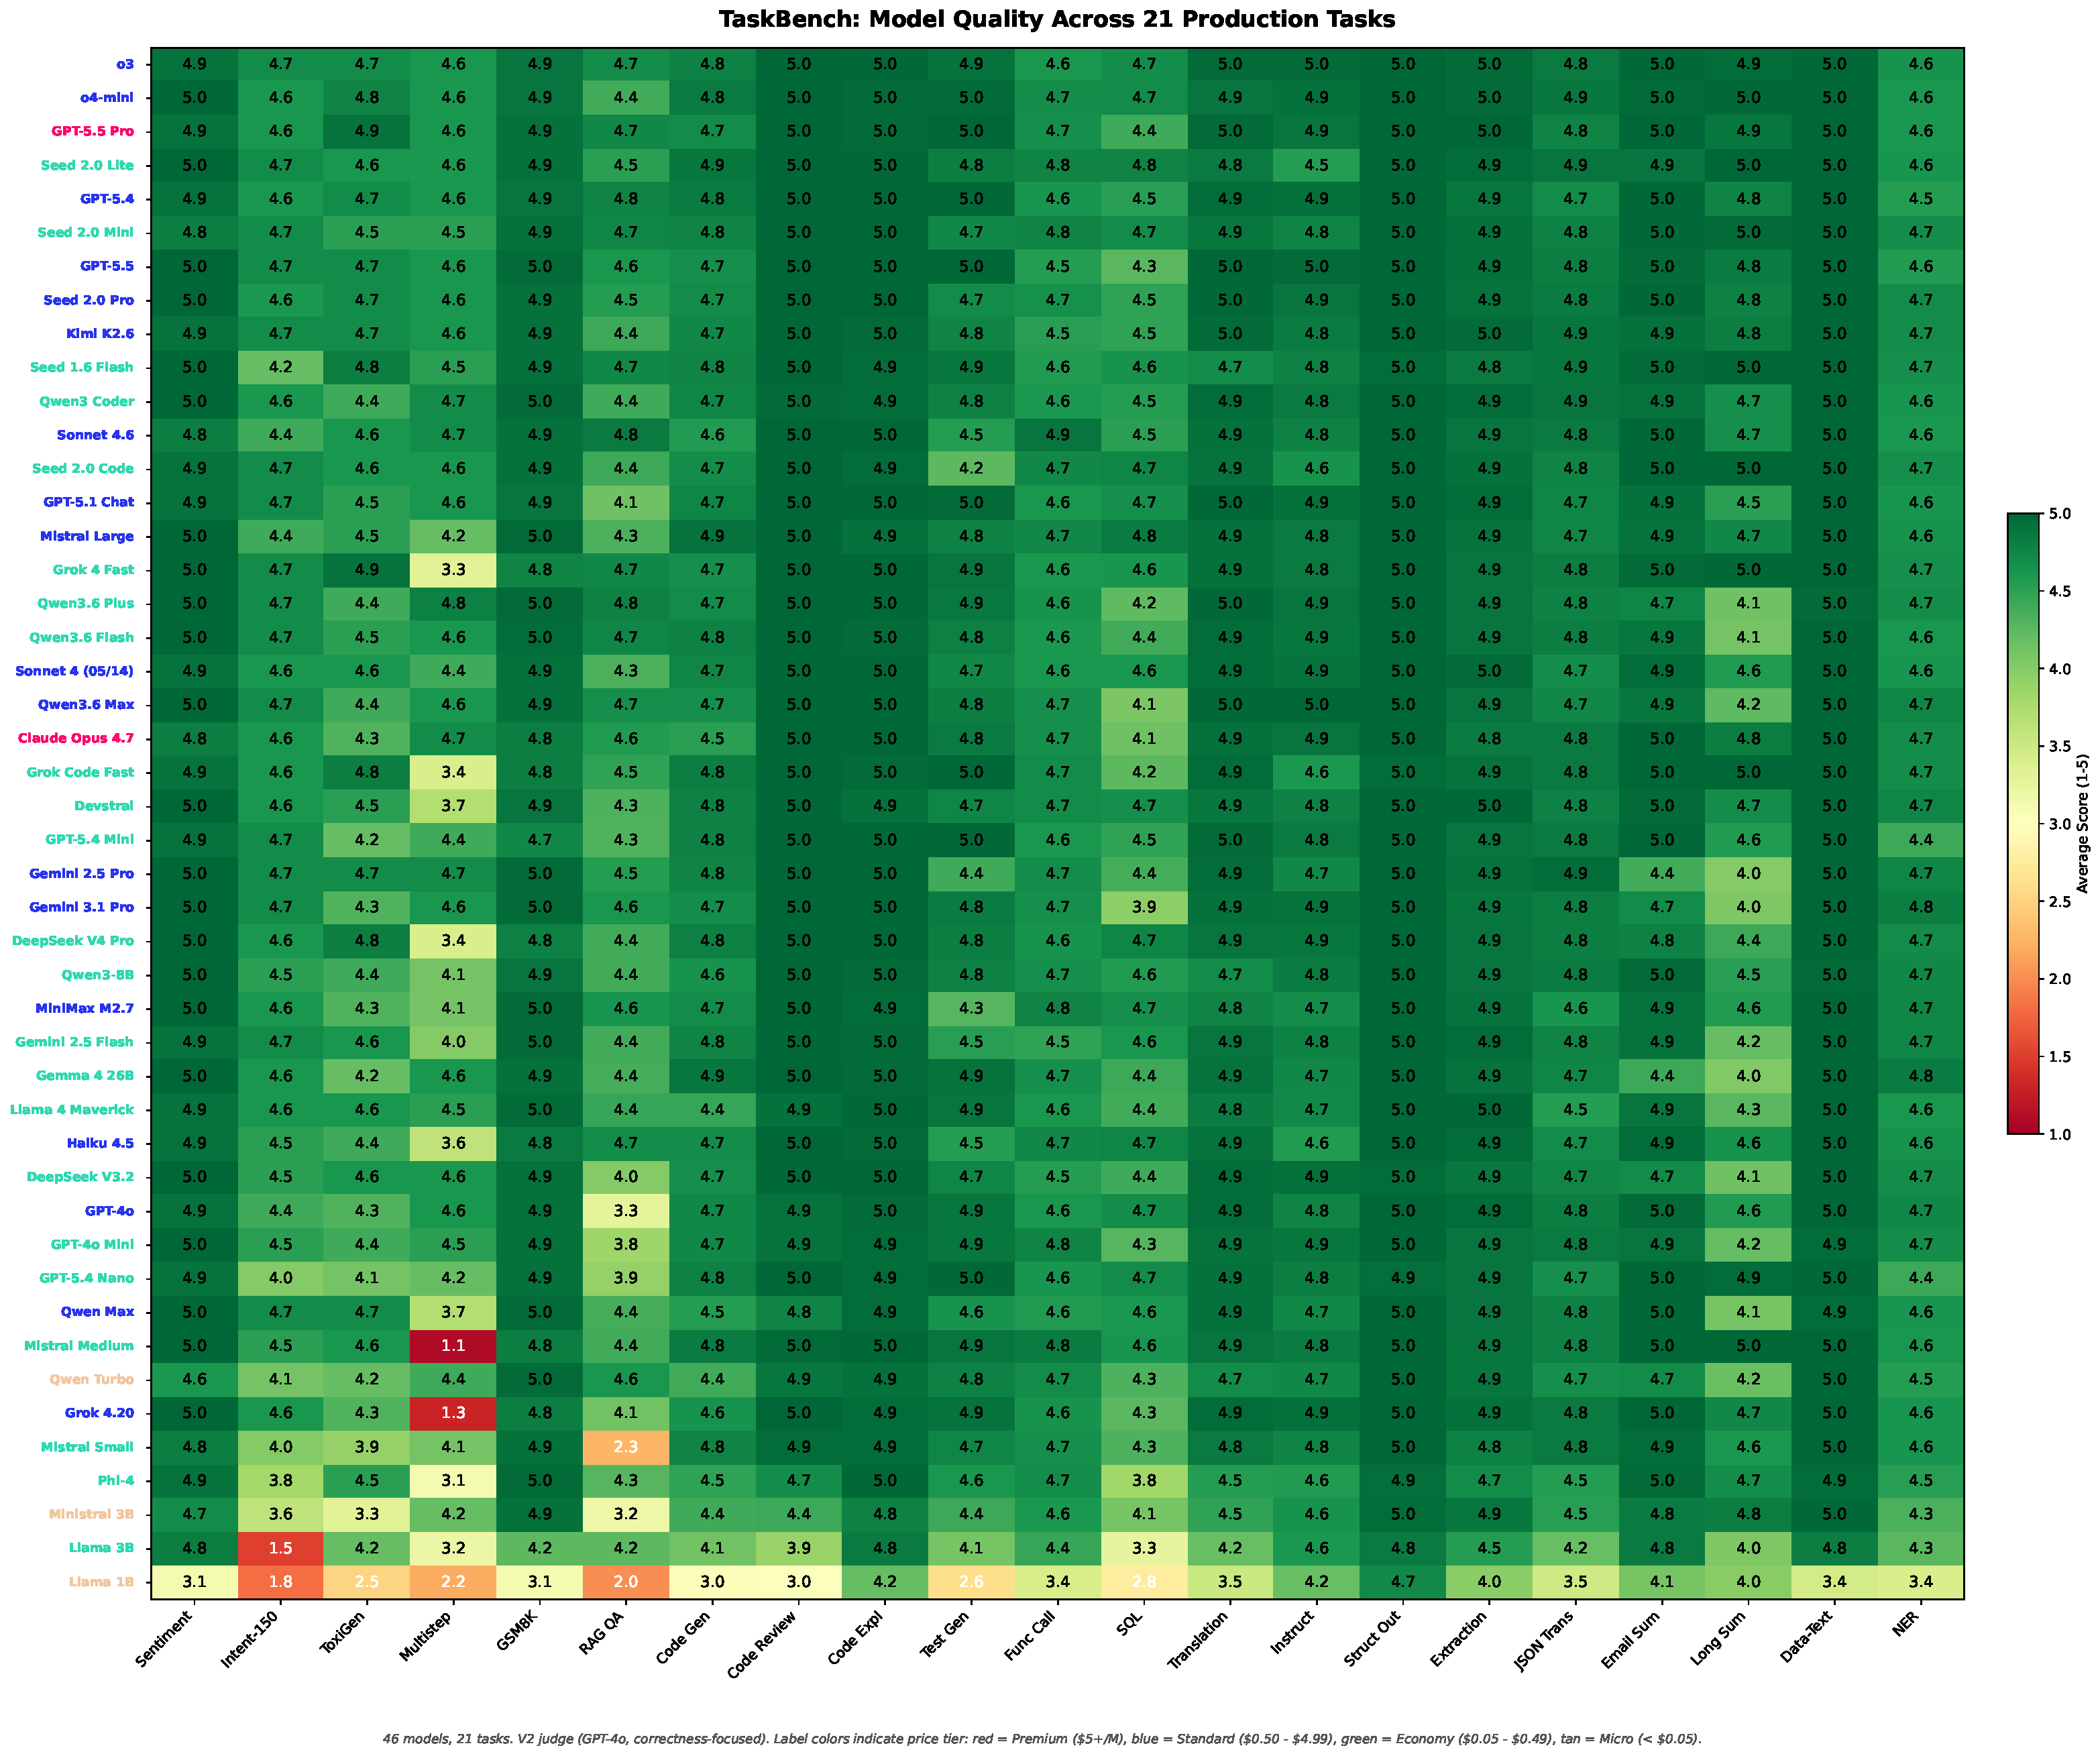
\includegraphics[width=\textwidth]{figures/heatmap_v3}
\caption{Quality heatmap (46 models $\times$ 21 tasks).  Rows sorted by
average score, columns grouped by task category.  Color intensity
indicates mean score per (model, task) pair on the 1--5 scale.  Most
cells are dark (above 4.5), with visible variation concentrated in
classification and QA tasks.}
\label{fig:heatmap}
\end{figure}


\subsection{Tier Comparison: Economy Matches Premium}

Bootstrap 95\% confidence intervals per tier (aggregated across all
tasks):

\begin{center}
\small
\begin{tabular}{lccr}
\toprule
\textbf{Tier} & \textbf{Mean} & \textbf{95\% CI} & \textbf{$n$ (pairs)} \\
\midrule
Premium  & 4.791 & [4.729, 4.853] & 42  \\
Standard & 4.783 & [4.760, 4.805] & 399 \\
Economy  & 4.741 & [4.710, 4.768] & 441 \\
Micro    & 4.287 & [4.128, 4.449] & 84  \\
\bottomrule
\end{tabular}
\end{center}

The Premium-to-Economy gap is 0.050 points (1.0\% of the 1--5 scale).
Confidence intervals overlap heavily.  Mann-Whitney tests find no
significant difference on 19 of 21 individual tasks ($p > 0.05$).  The
two significant results go in opposite directions: Economy outperforms
Premium on multistep reasoning ($p = 0.029$) while Premium outperforms
Economy on instruction following ($p = 0.043$).  With 21 simultaneous
tests at $\alpha = 0.05$, one to two rejections are expected by chance.

Micro is the only tier with a large gap ($-0.50$ versus Premium).  This
is driven by the four Micro models, which include the two sub-3B models
in our sample (Llama~1B and Ministral~3B).

\textbf{Caveat.}  With $n = 2$ Premium models, the Mann-Whitney test has
low statistical power.  We report ``no difference detected,'' not ``tiers
are equal.''  A future benchmark with five or more Premium models could
detect a small gap.  Even if a gap exists, it is bounded below 0.14
(the difference between the upper CI of Premium and the lower CI of
Economy).

\begin{figure}[t]
\centering
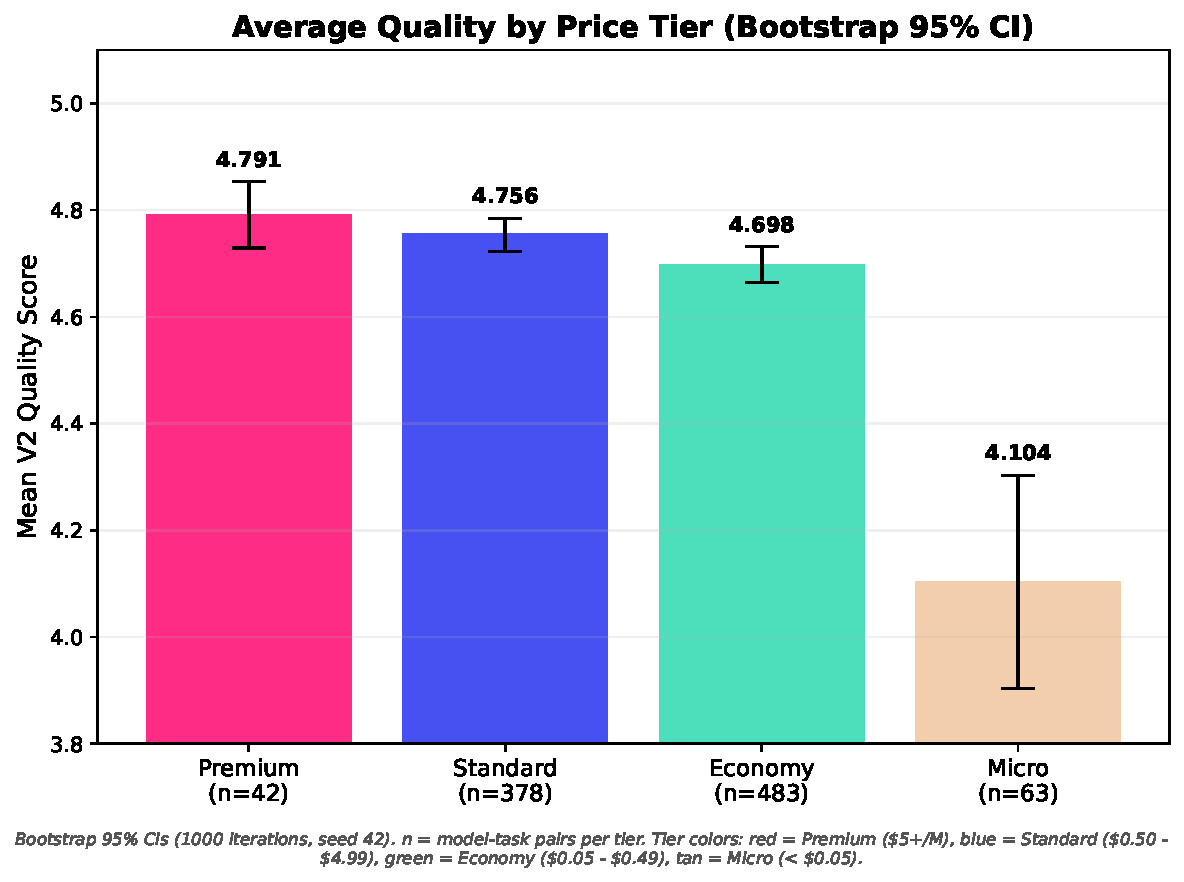
\includegraphics[width=0.6\textwidth]{figures/tier_comparison_v3}
\caption{Average quality by price tier with bootstrap 95\% confidence
intervals.  Premium and Economy intervals overlap on all 21 tasks.  Micro
is the only tier with a visible quality gap.}
\label{fig:tiers}
\end{figure}


\subsection{Per-Task Pareto Frontiers and Routing Savings}

For each task we compute the cost-quality Pareto frontier: the set of
models where no other model is both cheaper and higher quality.  Premium
models are almost never on the frontier.  The frontier is dominated by
Economy and Micro models.

Per-task routing to the cheapest model that matches o3 quality on each
task saves 99.7\% (\$0.003332/query for o3 alone versus
\$0.000009/query for the routed portfolio).  Even against the cheapest
single model covering all 21 tasks at the 4.5 threshold (Grok~4~Fast
at \$0.000435/query), routing saves approximately 98\%.

A portfolio of just four models covers all 21 tasks at the 4.0 quality
threshold: GPT-5.4~Nano on 16 tasks, Phi-4 on 3, Qwen Turbo on 1, and
Gemma~26B on 1.

\begin{figure}[t]
\centering
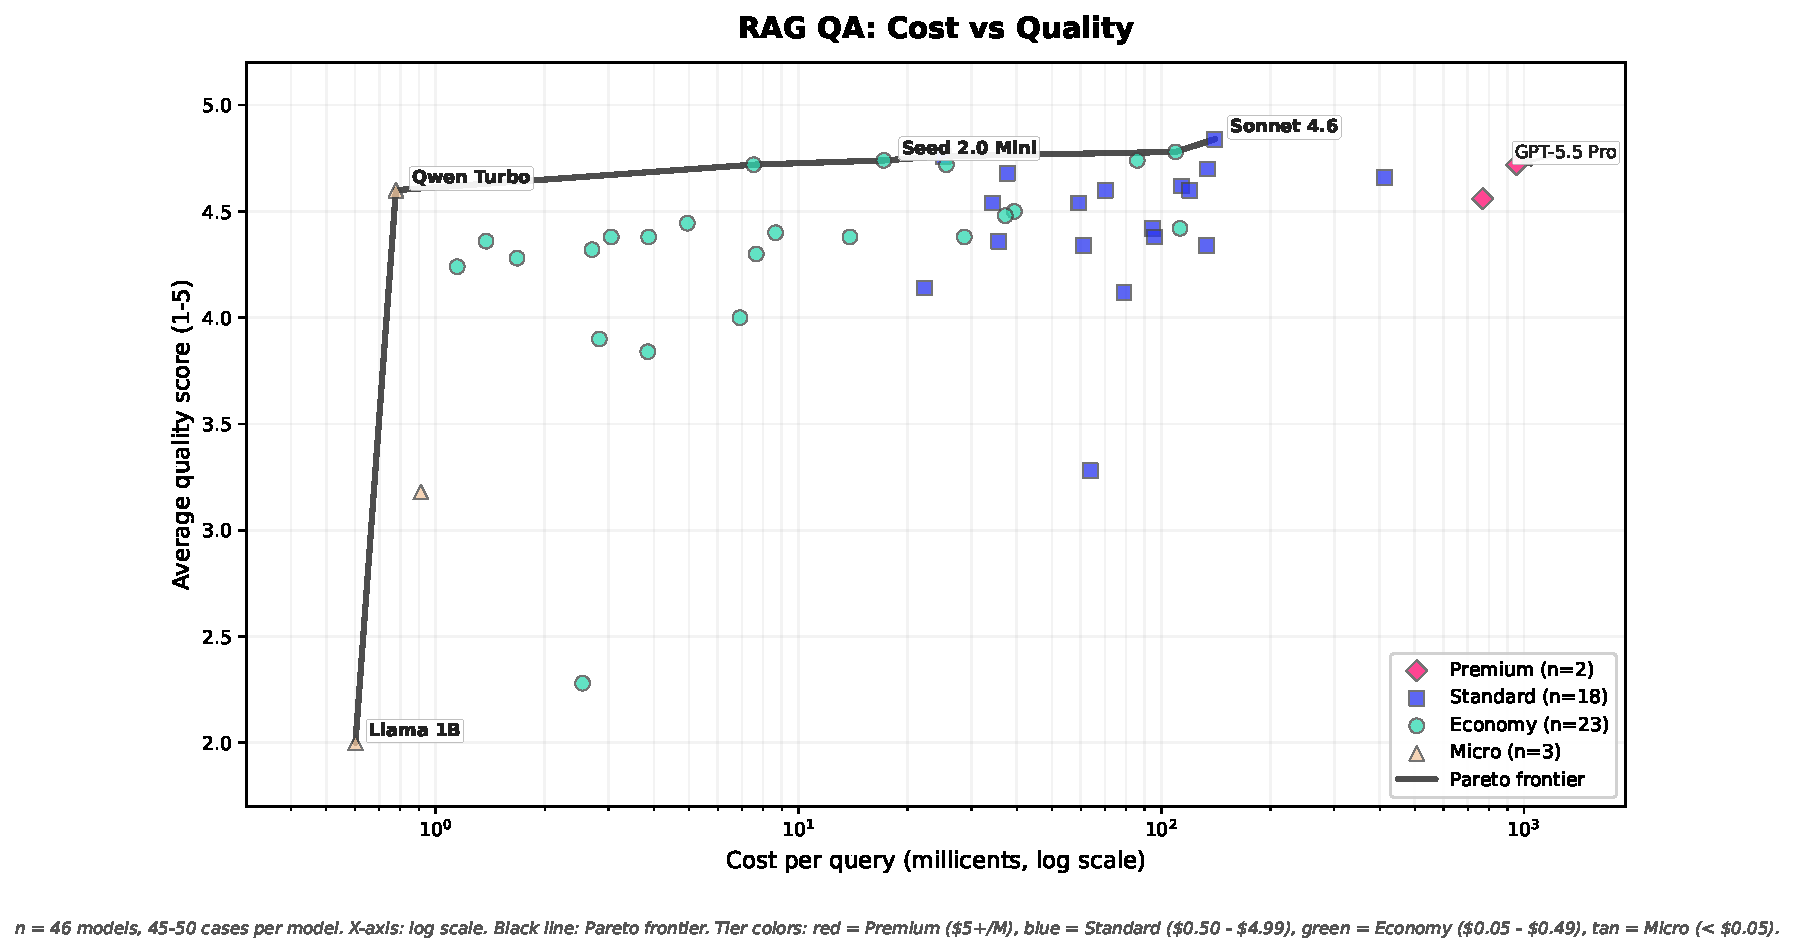
\includegraphics[width=\textwidth]{figures/pareto_rag_qa}
\caption{Pareto frontier for extractive QA (high-discrimination task,
log-scale cost axis).  Sonnet~4.6 dominates at 0.14\,mc; GPT-5.5~Pro
costs 7$\times$ more for lower quality.  Black line marks the Pareto
frontier.  Point shapes and colors indicate price tiers
(red\,=\,Premium, blue\,=\,Standard, green\,=\,Economy,
orange\,=\,Micro).}
\label{fig:pareto-rag}
\end{figure}

\begin{figure}[t]
\centering
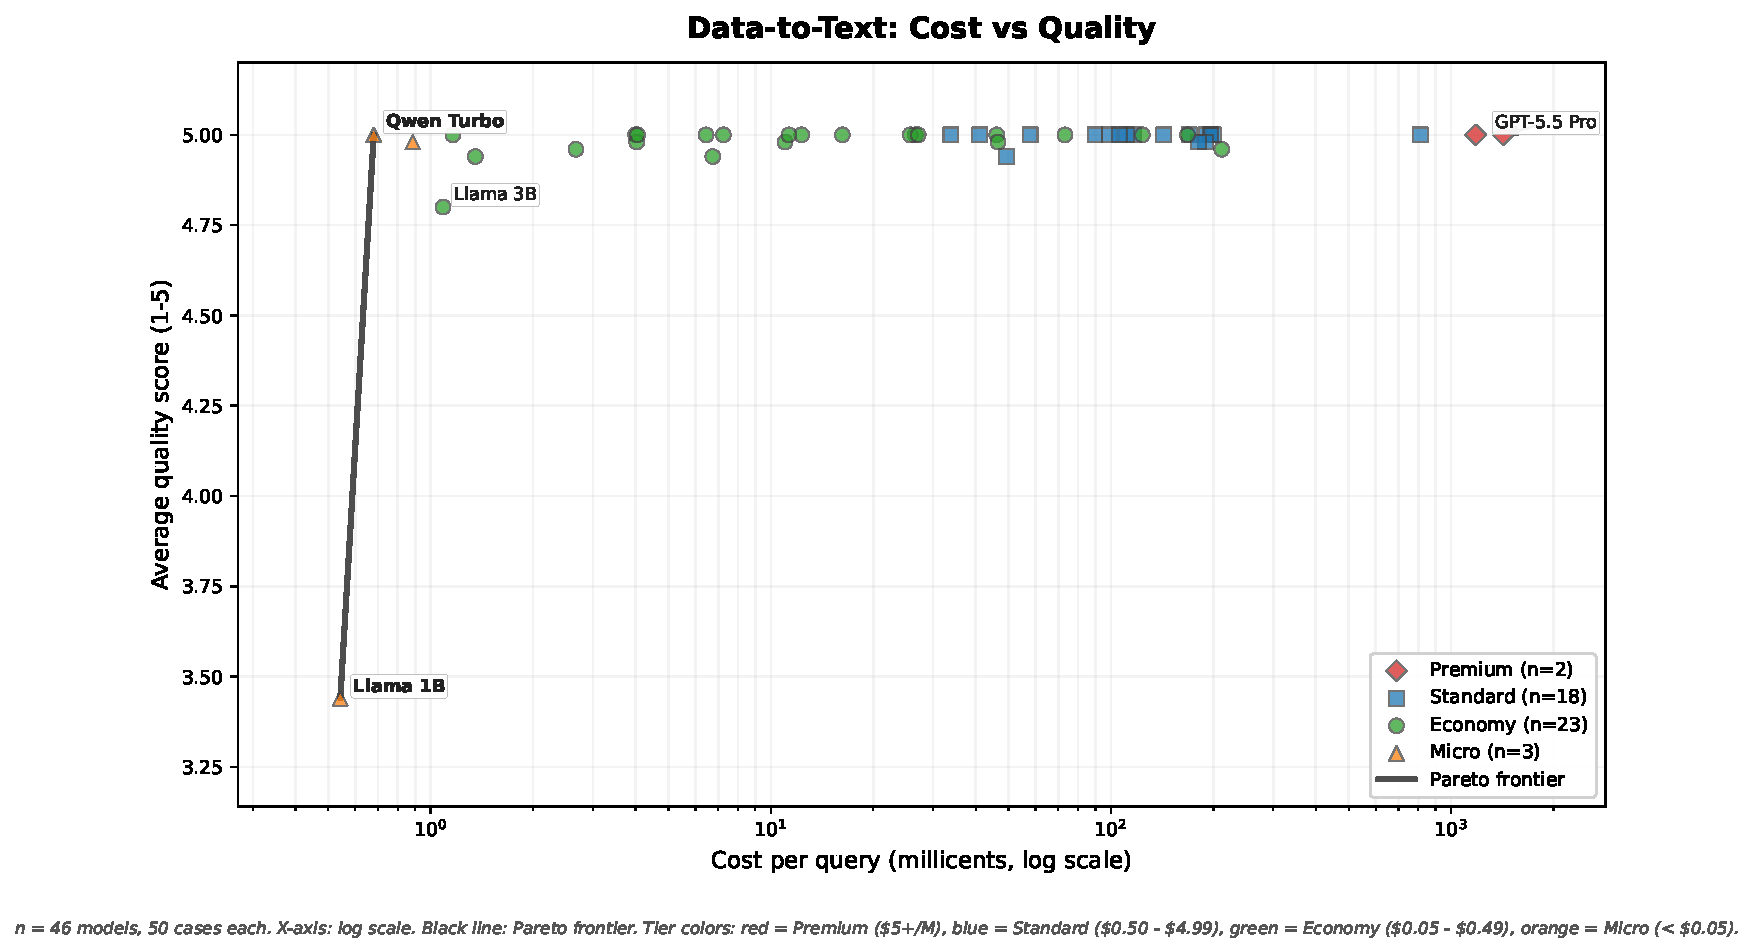
\includegraphics[width=\textwidth]{figures/pareto_data_to_text}
\caption{Pareto frontier for data-to-text (commodity task, log-scale
cost axis).  Qwen~Turbo achieves a perfect 5.0 at 0.0007\,mc; 30+
models match that score at up to 2{,}000$\times$ the cost.  The
near-flat frontier illustrates a task where model selection is
cost-irrelevant.}
\label{fig:pareto-data}
\end{figure}


\subsection{Provider Gradient: Paying More Buys Little}

Within each major provider, the most expensive model is not reliably the
best.

\textbf{Anthropic.}  Haiku at \$0.80/M scores 4.775.  Opus at \$15/M
scores 4.753.  Paying 19$\times$ more yields $-0.022$ quality.

\textbf{Google.}  Flash at \$0.15/M scores 4.749.  Pro at \$1.25/M
scores 4.747.  An 8$\times$ price increase yields $-0.002$.

\textbf{OpenAI.}  Nano at \$0.02/M scores 4.694.  GPT-5.5~Pro at
\$15/M scores 4.828.  A 750$\times$ price increase yields $+0.134$, the
largest intra-provider gain in our data, and still only 2.7\% of the
scale.

\textbf{Qwen.}  Turbo at \$0.05/M scores 4.654.  Max at \$2.00/M scores
4.746.  A 40$\times$ price increase yields $+0.092$.

\textbf{Mistral.}  Ministral~3B at \$0.04/M scores 4.441.  Large at
\$2.00/M scores 4.800.  A 50$\times$ price increase yields $+0.359$,
the only provider where paying more substantially helps.  This is driven
by the sub-3B model floor: Ministral~3B is the smallest model in our
benchmark.

The gradient is flat at the Standard/Economy boundary.  The only steep
segment is from Micro to Economy, driven by sub-3B models pulling the
Micro average down.

\begin{figure}[t]
\centering
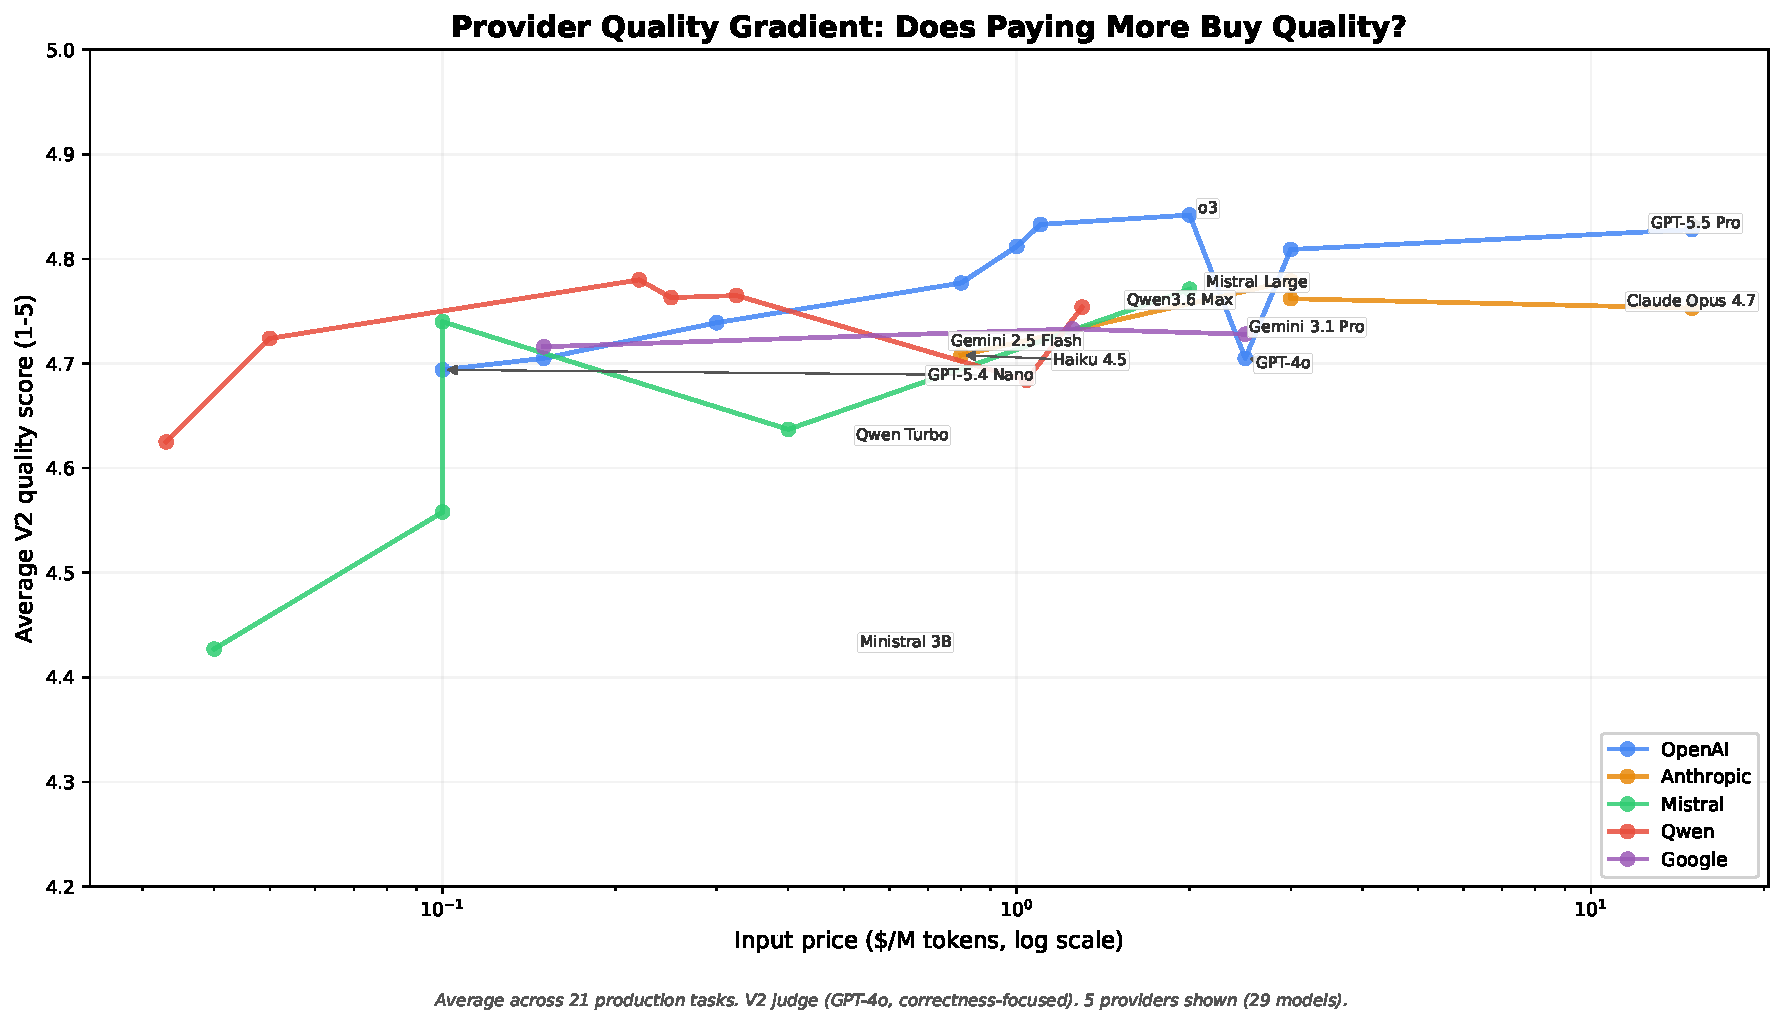
\includegraphics[width=0.85\textwidth]{figures/provider_gradient}
\caption{Within-provider price-quality gradient.  Each line connects
models from the same provider, ordered by input price.  The gradient is
nearly flat for Anthropic, Google, and Qwen.  OpenAI shows the largest
absolute gain ($+0.13$) across its 750$\times$ price range.  Mistral is
the exception, driven by its sub-3B entry-level model.}
\label{fig:gradient}
\end{figure}


\subsection{Model Selection in Practice}

Given that within-provider price increases yield minimal quality returns,
which models should a practitioner actually choose?

\paragraph{Coverage thresholds.}
At the 4.0/5 quality threshold, 37 of 46 models cover all 21 tasks.
Model choice barely matters.  At the 4.5 threshold, only five models
qualify as universal: Grok~4~Fast, Seed~2.0~Mini, GPT-5.4, Seed~2.0~Lite,
and o3.  The cheapest is Grok~4~Fast at \$0.000435/query average.  At
the 4.7 threshold, no single model covers all 21 tasks.  The bottleneck
tasks are extractive QA, intent detection, and content moderation.

\paragraph{Generational upgrades.}
The cost-quality frontier moves with each model generation.
GPT-4o to GPT-5.4: $-60$\% price (\$2.50 $\to$ \$1.00/M), $+0.089$
average quality.  GPT-4o Mini to GPT-5.4 Mini: $-33$\% price, quality
flat (already near ceiling).  Sonnet~4 to Sonnet~4.6: same price,
$+0.003$ quality.  The exception is DeepSeek V3.2 to V4~Pro:
$+211$\% price for $+0.061$ quality.  In three of four provider
families, the new generation is cheaper at equal or better quality.
Upgrading generations is a more reliable strategy than upgrading tiers.


% ============================================================
% 5. DISCUSSION
% ============================================================
\section{Discussion}

\subsection{Practical Implications}

Three recommendations for practitioners:

\begin{enumerate}[leftmargin=*,itemsep=2pt]
\item \textbf{Default to Economy tier.}  On 19 of 21 tasks, Economy
  models showed no significant quality difference versus Premium (the
  two exceptions favor opposite tiers).  The safest default is the
  cheapest model scoring at least 4.5 on the target task.
\item \textbf{Route per task for maximum savings.}  A four-model
  portfolio covers all 21 tasks at the 4.0 threshold and costs
  \$0.000009/query average.  The savings come from commodity tasks where
  Micro-tier models suffice.
\item \textbf{Upgrade generations, not tiers.}  GPT-5.4 is 60\% cheaper
  than GPT-4o at higher quality.  The cost-quality frontier moves
  down-left with each generation.  Paying for a premium tier within the
  same generation has near-zero return.
\end{enumerate}

Premium models may add marginal value on open-ended language tasks, but
the effect size ($< 0.2$ points) is within our task-level confidence
intervals.

\subsection{Evaluation Methodology Implications}

The format bias finding (Section~\ref{sec:judge-validation}) generalizes
beyond this benchmark.  Any LLM-as-judge evaluation using generic ``rate
quality 1--5'' rubrics likely contains this bias.  We recommend three
practices: (1) always validate against ground truth on at least two task
types, (2) use task-specific correctness anchors rather than generic
quality rubrics, and (3) report both judge scores and native metrics
where available.

Verbosity is not the primary driver of the bias ($r = 0.22$, $p = 0.13$
between verbosity ratio and V1-to-V2 score delta).  The mechanism is
rubric ambiguity: generic rubrics allow the judge to reward format
features that correlate with model price tier.


% ============================================================
% 6. LIMITATIONS
% ============================================================
\section{Limitations}
\label{sec:limitations}

\begin{itemize}[leftmargin=*,itemsep=3pt]

\item \textbf{$n = 2$ Premium models.}  The Economy-matches-Premium
  finding is ``no difference detected,'' not ``tiers are equal.''  Two
  Premium models (Claude Opus~4.7 and GPT-5.5~Pro) provide low
  statistical power.  Future work should include five or more Premium
  models.

\item \textbf{Judge validated on 3 of 17 LLM-judged tasks.}  The
  remaining 14 tasks are validated by mechanism consistency (identical
  rubric structure and GPT-4o judge), not by direct ground-truth
  correlation.

\item \textbf{50 cases per task.}  Confidence intervals are approximately
  $\pm 0.2$.  Differences below 0.3 are not distinguishable from noise.
  This is standard for benchmark papers; HELM uses similar per-scenario
  sample sizes.

\item \textbf{Single-turn only.}  Multi-turn conversations, vision, and
  audio inputs are out of scope.

\item \textbf{Price snapshot (April--May 2026).}  LLM prices change
  monthly.  Tier-level findings are more durable than absolute prices
  because relative pricing between tiers rarely inverts.  We release raw
  data for re-computation with current prices.

\item \textbf{Potential data contamination.}  Models may have seen
  GSM8K, SQuAD, and HumanEval during training.  This affects absolute
  scores but not relative comparisons, since all models face the same
  contamination risk on standard datasets.

\item \textbf{Reasoning model cost tracking.}  GPT-5.5~Pro and o3
  reasoning tokens are partially invisible in the API response.  Tracked
  cost (\$143.81 total spend) underestimates real spend (approximately
  \$180+) for these models specifically.  Non-reasoning model costs
  remain accurate.

\item \textbf{Model diversity.}  Our sample includes three geographic
  origins and both open-weight and closed-source licenses.  Neither
  dimension significantly predicts quality: provider origin shows no
  effect (Kruskal-Wallis $H = 1.83$, $p = 0.40$), and the
  open-versus-closed gap (0.183, $p = 0.0004$) is driven by sub-3B
  open-weight models (see Appendix~\ref{app:diversity}).

\item \textbf{English-only} (except the EN$\to$FR translation task).

\end{itemize}


% ============================================================
% 7. CONCLUSION
% ============================================================
\section{Conclusion}

TaskBench provides a systematic per-task cost-quality benchmark for
production LLM use.  Across 46 models and 21 tasks, we find that the
cost-quality curve is flat: on 19 of 21 tasks we detect no significant
difference between Economy and Premium tiers, and the two significant
results favor opposite tiers ($n_{\text{Premium}} = 2$; more Premium
models are needed to confirm this pattern).  The practical
implication is that practitioners should default to Economy models and
use per-task routing for maximum savings.

We also show that standard LLM-as-judge evaluation has a format bias that
specifically distorts cost-quality comparisons.  Correctness-focused
rubrics fix this with minimal effort.

We release all 51{,}580 scored cases, 51{,}705 raw model responses,
evaluation prompts, and analysis code.  We encourage the community to
extend TaskBench with more Premium models, multi-turn tasks, and
longitudinal price tracking.


% ============================================================
% ACKNOWLEDGMENTS + DISCLOSURE
% ============================================================
\section*{Acknowledgments and Disclosure}

\textbf{Disclosure.}  This work was conducted by S\'{e}bastien Conejo,
co-founder of Manifest (\url{https://github.com/mnfst/manifest}), an
open-source LLM model router.  Manifest was not used in this benchmark.
The routing savings analysis (Section~4.3) applies to any routing system
and is computed from the benchmark data using a simple per-task argmin.
All code, data, and evaluation prompts are publicly available.\footnote{\url{https://github.com/SebConejo/benchmark-reverse-engineering}}


% ============================================================
% BIBLIOGRAPHY
% ============================================================
\bibliography{references}


% ============================================================
% APPENDIX
% ============================================================
\appendix

\section{Full Pareto Frontiers (21 Tasks)}
\label{app:pareto}

One single-panel log-scale Pareto figure per task, following the style of
Figures~\ref{fig:pareto-rag} and~\ref{fig:pareto-data}.  Figures are
available in \texttt{results/figures/} in the companion repository.

% Placeholder: include all 21 Pareto PNGs during formatting.
% \foreach \task in {sentiment_sst2, intent_clinc150, ...} {
%   \includegraphics[width=\textwidth]{../results/figures/pareto_\task}
% }


\section{Complete Model Table}
\label{app:models}

Table with all 46 complete models: provider, model name, price tier,
input price/M, output price/M, average score, rank, and number of valid
cases.  Available as \texttt{task\_model\_aggregates.json} in the
companion repository.

% Full table to be inserted during formatting.


\section{Judge Validation Details}
\label{app:judge}

V1 versus V2 correlation summaries for all four validated task types:

\begin{center}
\small
\begin{tabular}{llccl}
\toprule
\textbf{\#} & \textbf{Task} & \textbf{V1 $r$} & \textbf{V2 $r$} & \textbf{Native metric} \\
\midrule
1 & Math reasoning (GSM8K)  & 0.388  & 0.905 & Numerical accuracy \\
2 & Extractive QA (SQuAD)   & $-0.013$ & 0.888 & Substring match \\
3 & Code generation (HumanEval) & 0.491\textsuperscript{*} & 0.891 & pass@1 \\
4 & Translation (OPUS-100)  & n/a    & 0.290 & BLEU (single ref.) \\
\bottomrule
\end{tabular}
\end{center}
\textsuperscript{*}V1 code correlation uses a naive harness; V2 uses the
multi-strategy harness.

The code generation validation required a multi-strategy test harness.
A naive harness using \texttt{textwrap.indent} failed on 47.2\% of
responses due to indentation mismatches.  Our multi-strategy approach
tries four extraction strategies in sequence (standalone function
extraction, uniform indent, selective indent, raw append), resolving
91.4\% of formatting failures and raising the pass rate from 44.9\% to
91.4\%.

Translation BLEU is inconclusive ($r = 0.29$) due to the metric's
single-reference limitation, not the judge's quality.

Per-task ranking flip rates range from 20.2\% (code review, Kendall
$\tau = 0.596$) to 50.3\% (extractive QA, $\tau = -0.006$).  The
aggregate flip rate is 34.7\% (5{,}195 of 14{,}972 pairs).

% Full score-distribution shift tables and scatter plots to be added.


\section{Judge Prompts}
\label{app:prompts}

Full V1 and V2 judge prompt text for all 17 LLM-judged tasks.  Available
in \texttt{JUDGE\_PROMPTS\_V2.md} in the companion repository.


\section{Statistical Tables}
\label{app:stats}

Bootstrap 95\% confidence intervals per (task, tier) and Mann-Whitney $U$
$p$-values per task (Economy versus Premium, Economy versus Standard).
Coverage matrix showing per-model threshold coverage at 4.0, 4.5, and
4.7.  Per-task routing savings (cheapest adequate model, cost, and
savings percentage).  All data available in
\texttt{results/analysis\_v3\_final/} in the companion repository.


\section{Top-5 Models Per Task}
\label{app:top5}

For each of the 21 tasks, the five highest-scoring models ranked by
quality (ties broken by lowest cost).  Available as
\texttt{top5\_per\_task.json} in the companion repository.


\section{Model Diversity Analysis}
\label{app:diversity}

\paragraph{Provider origin.}
Three geographic groups: Chinese ($n = 16$, mean 4.779), American
($n = 26$, mean 4.682), and European ($n = 5$, mean 4.691).
Kruskal-Wallis $H = 1.83$, $p = 0.40$.  No significant difference.  The
American group has the widest range (3.394 to 4.842), driven by sub-3B
Llama models at the low end.

\paragraph{License type.}
Open-weight ($n = 18$, mean 4.603) versus closed-source ($n = 30$, mean
4.786).  Mann-Whitney $p = 0.0004$, gap 0.183.  However, the open-weight
group includes all sub-3B models (Llama~1B, Llama~3B, Ministral~3B).
Excluding sub-3B models narrows the gap to approximately 0.066.  The
license effect is driven primarily by model size, not by the open-weight
development process.


\section{Task Discriminativeness}
\label{app:discriminativeness}

Horizontal bar chart showing score spread (maximum minus minimum) per
task across all 46 models, with tasks color-coded by category.  Available
as \texttt{task\_discriminativeness\_v3.svg} in the companion repository.


\end{document}
